\documentclass{IEEEtran}

\usepackage{graphicx}
\usepackage{caption}
\usepackage{subcaption}
\usepackage{hyperref}
\usepackage{url}

\bibliographystyle{plain}

\begin{document}

\title{Computational Psycholinguistics --- Assignment 2}
\author{Daan Brugmans (S1080742)}
\date{\today}

\graphicspath{{./images}}

\maketitle

\section{Introduction}
This report is the realization of the Assignment 2 project for the Radboud University course \href{https://www.ru.nl/courseguides/arts/courses/ma/rema-lc/let-rema-lcex28/}{Computational Psycholinguistics}.
For this assignment, students must investigate whether the gradients computed from a recurrent neural network correlate with measured P600 component activity from a controlled experiment.
The reasoning behind this assignment is that recent research (\cite{fitz2019erp,frank2024gradients}) has shown that the P600 component may be the backpropagation of prediction errors in the human language system.
Since neural language models also backpropagate their prediction errors using gradients, there may exist similarities between the language error backpropagation of human and artificial neural language systems.
This report contains the findings found by me for the Assignment 2 project.

The relevant code for this assignment can be found at the following URL: \url{https://github.com/daanbrugmans/ru-computational-psycholinguistics-23-24/tree/main/assignment-2/code}.

\section{Related Work}
For my realization of Assignment 2, I have chosen a controlled experiment from \cite{kim2005combinatory}, specifically their first experiment.
Kim and Osterhout researched P600 activity in anomalous sentences.
When they released their research, it was generally accepted that the P600 component was solely responsible for language error related to syntax, while the N400 was responsible for language error related to semantics.
In their work, Kim and Osterhout show that the P600 is still activated in sentences that are syntactically unambiguous, but have illogical semantics as a result, however.
The general structure of such sentences was one where the two agents of a sentence are swapped, maintaining a certain "theme" and a valid syntax, while going against semantics that are considered regular.
An example of this is the sentence "\textit{The hearty meal was devouring the kids}", where the syntax is unambiguous, but does imply a meaning that goes against what is usually expected of the combination of the sentence's agents and theme, which would be "\textit{The kids were devouring the hearty meal}".
The authors name such sentences \textbf{(Attraction) Violations}.

Kim and Osterhout note that Attraction Violations, especially the phrase up and including the critical verb ("\textit{The hearty meal was devouring}"), while syntactically unambiguous, can be interpreted to be either syntactically or semantically incorrect.
If a reader interprets the violation as syntactically invalid, then they likely think that the critical verb is in the wrong tense, and changing it would return the sentence to a meaning that aligns with expectations ("\textit{The hearty meal was devoured}").
If a reader interprets the violation as semantically invalid, then they likely think that the agent is wrong, and, in the case of the full sentence, that the agents should be flipped ("\textit{The kids were devouring}").
This means that an Attraction Violation can cause a syntactically unambiguous sentence to be considered syntactically invalid due to its semantics.
On the basis of this phenomenon, Kim and Osterhout researched if sentences with Attraction Violations can trigger a P600 effect in humans.
Although P600 effects were typically taken to be responsible for purely syntactic errors at that time, syntactically unambiguous Attraction Violation sentences, which can be considered to be syntactically erroneous on the basis of the sentences meaning, may thus elicit a P600 response based on a sentence's unexpected semantics.

\begin{figure}
    \centering
    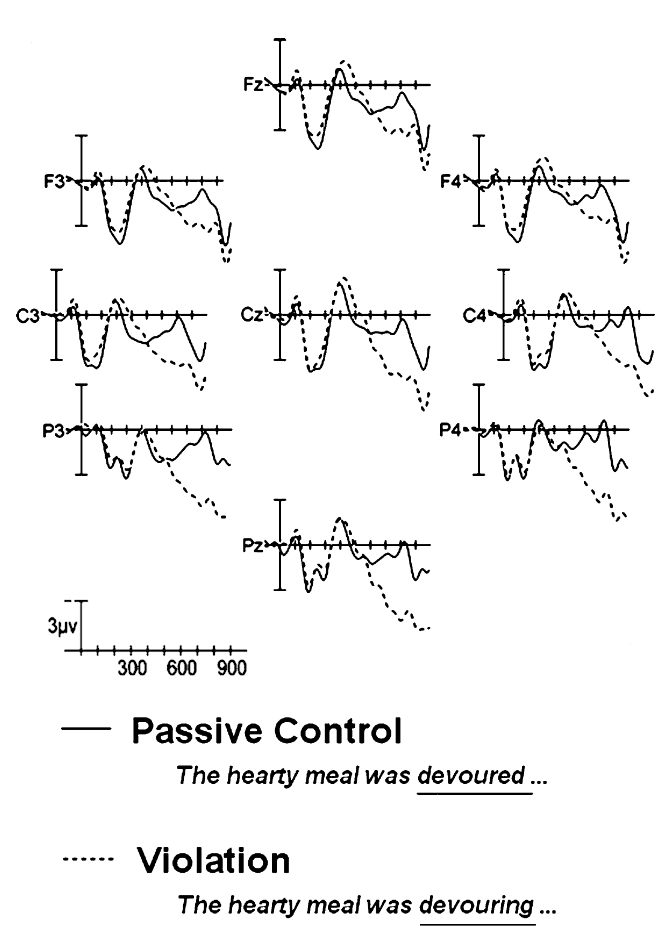
\includegraphics[width=.45\textwidth]{kim_osterhout.png}
    \caption{ERP Brain Activity when reading Violation vs. Control sentences, from \cite{kim2005combinatory}.}
    \label{fig:kim_osterhout}
\end{figure}

Kim and Osterhout conduct an experiment where participants' N400 and P600 components are read while reading both Attraction Violation sentences ("\textit{The hearty meal was devouring}"), and Control Sentences where the critical verb of the sentence is altered as to let the sentence be both syntactically and semantically coherent with its agents and theme ("\textit{The hearty meal was devoured}").
Their results show that, on the critical verb, the P600 component is much more pronounced on Attraction Violation sentences than on the Control sentences.
They also showed that the N400 component is only slightly present when Attraction Violation sentences are read, meaning that the error stemming from the sentence is mostly processed by the P600.
These findings then imply that the P600 is not responsible for syntactic error alone, and that a degree of semantic error is also processed in the P600.
A visualization of these findings can be seen in figure \ref{fig:kim_osterhout}.

\section{Methodology}
All the code I have written can be found in the Jupyter Notebook called \texttt{main.ipynb}, which should thusly contain all results also shown in this report.
It can be found at the following URL: \url{https://github.com/daanbrugmans/ru-computational-psycholinguistics-23-24/blob/main/assignment-2/code/main.ipynb}
I have placed the code in the \texttt{get\_predictions.py} file in a function called \texttt{get\_predictions}, so that I can easily call this code from the notebook.

Kim and Osterhout (\cite{kim2005combinatory}) provide their full set of Attraction Violation sentences and (Passive) Control sentences in their paper.
I have copied the full sets of these sentences up until and including the critical verb.
I have stored them as text files called \texttt{violations.txt} for the Attraction Violation sentences and \texttt{control.txt} for the Control sentences in a folder called \texttt{data}.
The notebook processes these sentences further so that they can be used by the RNNs by lowercasing all words and separating genitive markers ('s) from consonants.
Furthermore, after the surprisals and gradients have been calculated, I remove sentences that do not have surprisal and/or gradient information, and remove sentence-initial words from sentences that do.

My results are a collection of scatterplots that visualize the relationship between the surprisal and gradients of the models.
Every plot also contains a quadratic function fitted to the data to show the trend of the relationship between the variables.
I have chosen for a quadratic function as opposed to a linear function, as I found that this fits the data better.
Included in every plot is also the Pearson Correlation Coefficient \textit{r} between variables.
Since surprisal values and gradients are calculated for multiple models, I provide a plot for every model.
For every pair of variables, I also provide a plot of how the Pearson Correlation Coefficient changes as the model is trained on more data.

Before producing results, I set a universal seed for Python itself, NumPy, and PyTorch of \texttt{3131}.
I do this in order to improve the reproducibility of my results.
This is why I also set some settings for CUDA regarding PyTorch's randomness when computing on GPU.

\section{Results}
% \begin{figure*}
%     \centering
%     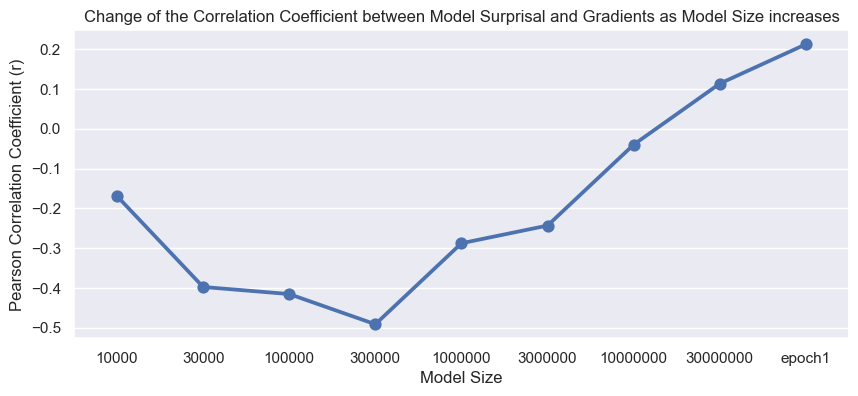
\includegraphics[width=.9\textwidth]{correlation_change/surprisal_gradients.png}
%     \caption{The change of the Pearson Correlation Coefficient between Model Surprisal and Model Gradients as the model is trained on increasingly more data.}
%     \label{fig:coefficient_surprisal_gradients}
% \end{figure*}
% \begin{figure*}
%     \centering
%     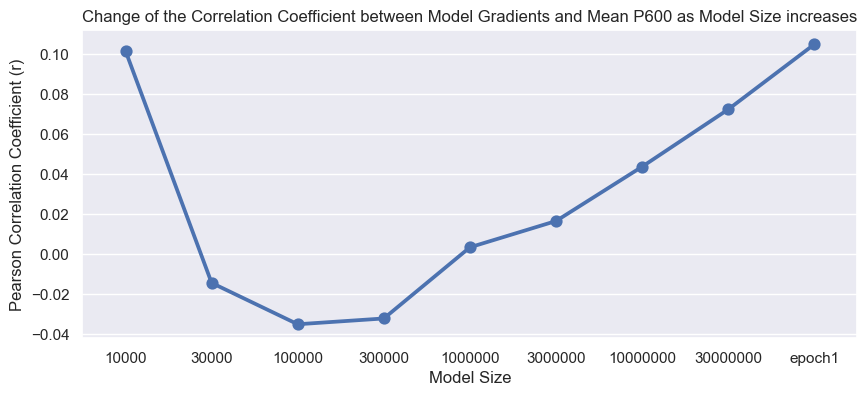
\includegraphics[width=.9\textwidth]{correlation_change/gradients_p600.png}
%     \caption{The change of the Pearson Correlation Coefficient between Model Gradients and P600 as the model is trained on increasingly more data.}
%     \label{fig:coefficient_gradients_p600}
% \end{figure*}
% \begin{figure*}
%     \centering
%     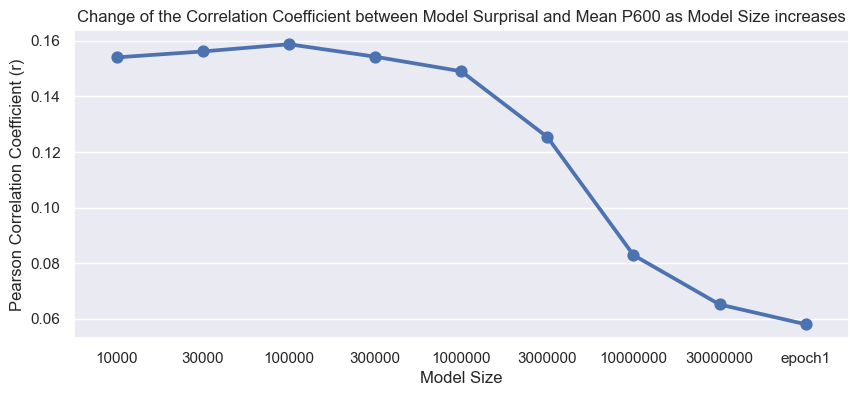
\includegraphics[width=.9\textwidth]{correlation_change/surprisal_p600.png}
%     \caption{The change of the Pearson Correlation Coefficient between Model Surprisal and Mean P600 as the model is trained on increasingly more data.}
%     \label{fig:coefficient_surprisal_p600}
% \end{figure*}

% Figures \ref{fig:coefficient_surprisal_gradients}, \ref{fig:coefficient_gradients_p600}, and \ref{fig:coefficient_surprisal_p600} show the change of the correlation between variables as the amount of data the neural language model has trained on increases.
% The exact values of the points in this plot can be found in tables \ref{tab:correlation_surprisal_gradients}, \ref{tab:correlation_gradients_p600}, and \ref{tab:correlation_surprisal_p600} respectively.
% The individual scatterplots are placed in the appendices.
The full results can be found in the appendices, where the graphs for every model are shown for all four comparisons:
\begin{itemize}
    \item Violation vs. Control Surprisal
    \item Violation vs. Control Gradients
    \item Violation Surprisal vs. Control Surprisal
    \item Violation Gradients vs. Control Gradients
\end{itemize}

\subsection{Comparing Surprisal vs Gradients}
\begin{figure}
    \centering
    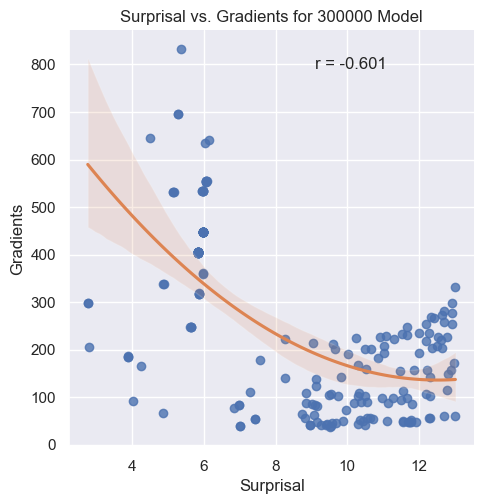
\includegraphics[width=.45\textwidth]{violations_surprisal_vs_gradients/300000.png}
    \caption{Surprisal vs. Gradients on Violations for an RNN trained on 300,000 sentences.}
    \label{fig:300000_surprisal_vs_gradients}
\end{figure}

\begin{figure*}
    \centering
    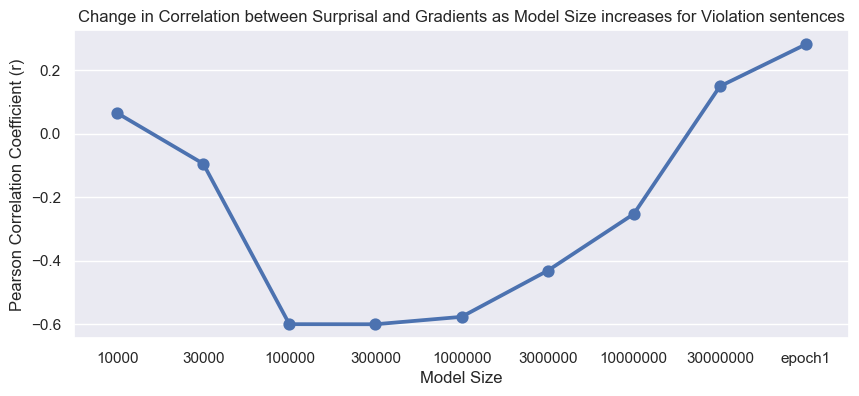
\includegraphics[width=.9\textwidth]{correlation_change/violations_surprisal_vs_gradients.png}
    \caption{The change in Correlation between Model Surprisal and Gradients on Violation Sentences as the model is trained on increasingly more data.}
    \label{fig:correlation_violations_surprisal_gradients}
\end{figure*}
\begin{figure*}
    \centering
    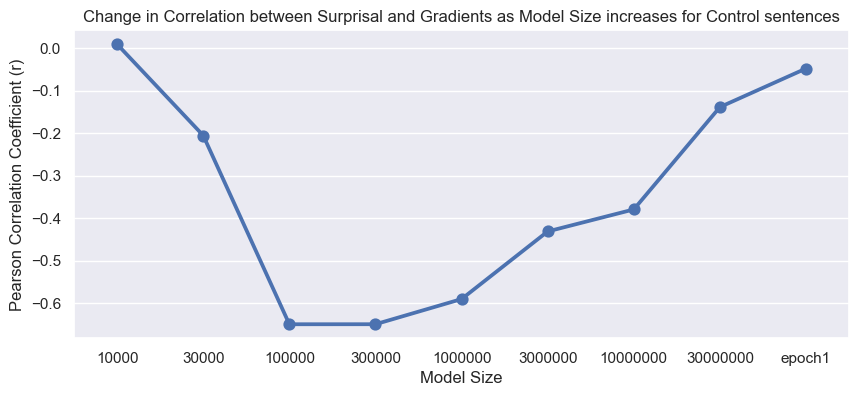
\includegraphics[width=.9\textwidth]{correlation_change/control_surprisal_vs_gradients.png}
    \caption{The change in Correlation between Model Surprisal and Gradients on Control Sentences as the model is trained on increasingly more data.}
    \label{fig:correlation_control_surprisal_gradients}
\end{figure*}

Figure \ref{fig:correlation_violations_surprisal_gradients} shows the change in Pearson Correlation Coefficient between a model's surprisal and gradients on sentences with an Attraction Violation as the model has been trained on more data.
Figure \ref{fig:correlation_control_surprisal_gradients} shows the same information, but for Control sentences.
Tables \ref{tab:correlation_violations_surprisal_gradients} and \ref{tab:correlation_control_surprisal_gradients} show the exact correlation coefficient values from these plots.
Finally, figure \ref{fig:300000_surprisal_vs_gradients} shows an example of a model's surprisals against its gradients, specifically the Recurrent Neural Network trained after 300,000 sentences.

\begin{table}
    \centering
    \begin{tabular}{c|c}
        \textbf{Trained Sentences Count} & \textbf{\textit{r}} \\
        \hline
        10,000&0.065\\
        30,000&-0.094\\
        100,000&-0.600\\
        300,000&-0.601\\
        1,000,000&-0.577\\
        3,000,000&-0.431\\
        10,000,000&-0.252\\
        30,000,000&0.149\\
        epoch1&0.282
    \end{tabular}
    \caption{Correlation Coefficients between Model Surprisal and Gradients on Violation Sentences by the model's train data size.}
    \label{tab:correlation_violations_surprisal_gradients}
\end{table}
\begin{table}
    \centering
    \begin{tabular}{c|c}
        \textbf{Trained Sentences Count} & \textbf{\textit{r}} \\
        \hline
        10,000&0.009\\
        30,000&-0.205\\
        100,000&-0.650\\
        300,000&-0.650\\
        1,000,000&-0.591\\
        3,000,000&-0.431\\
        10,000,000&-0.380\\
        30,000,000&-0.139\\
        epoch1&-0.048
    \end{tabular}
    \caption{Correlation Coefficients between Model Surprisal and Gradients on Control Sentences by the model's train data size.}
    \label{tab:correlation_control_surprisal_gradients}
\end{table}

\subsection{Comparing Conditions}
\begin{figure*}
    \centering
    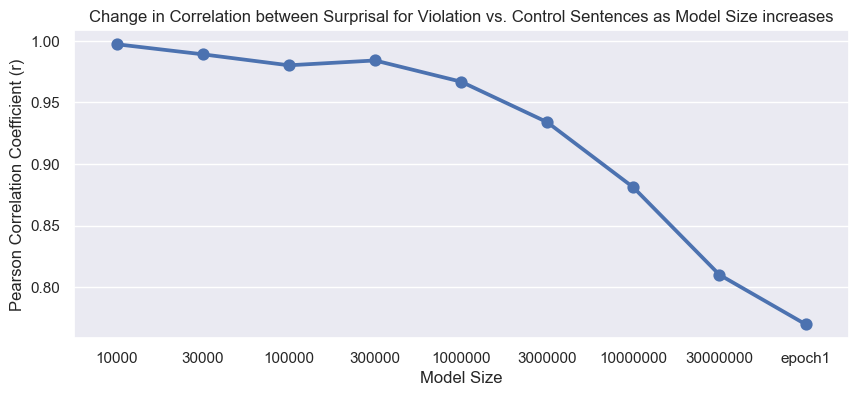
\includegraphics[width=.9\textwidth]{correlation_change/surprisal_violations_vs_control.png}
    \caption{The change in Correlation of Model Surprisal between Violation Sentences and Control Sentences as the model is trained on increasingly more data.}
    \label{fig:correlation_surprisal_violation_control}
\end{figure*}
\begin{figure*}
    \centering
    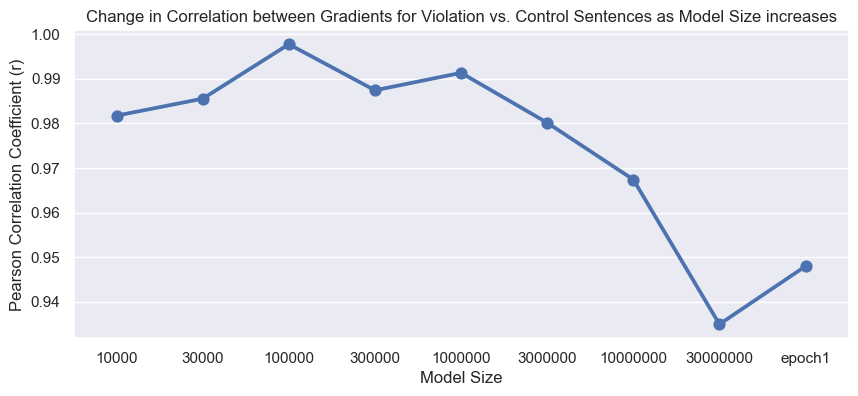
\includegraphics[width=.9\textwidth]{correlation_change/gradients_violations_vs_control.png}
    \caption{The change in Correlation of Model Gradients between Violation Sentences and Control Sentences as the model is trained on increasingly more data.}
    \label{fig:correlation_gradients_violation_control}
\end{figure*}

\begin{figure*}[h]
    \centering
    \begin{subfigure}{0.4\textwidth}
        \centering
        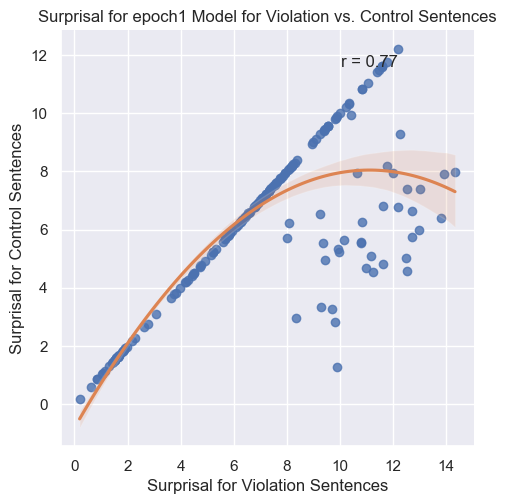
\includegraphics[width=\textwidth]{surprisal_violations_vs_control/epoch1.png}
    \end{subfigure}
    \begin{subfigure}{0.4\textwidth}
        \centering
        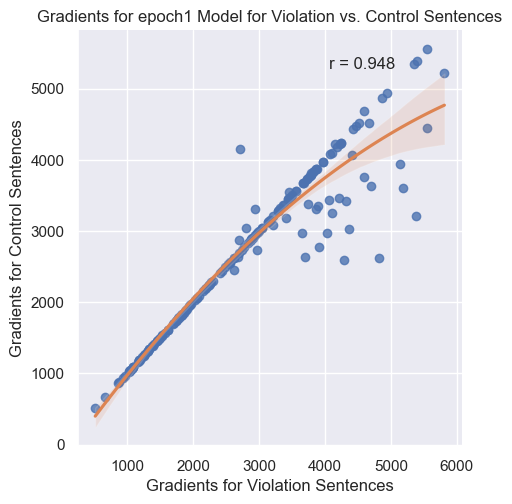
\includegraphics[width=\textwidth]{gradients_violations_vs_control/epoch1.png}
    \end{subfigure}
    \caption{Plots of the correlation between the fully trained (epoch1) model's surprisals (left) and gradients (right) on Violation Sentences vs. Control Sentences.}
    \label{fig:epoch1_correlations}
\end{figure*}

Figure \ref{fig:correlation_surprisal_violation_control} shows the change in Pearson Correlation Coefficient between a model's surprisal on sentences with an Attraction Violations versus Control sentences as the model has been trained on more data.
Figure \ref{fig:correlation_gradients_violation_control} shows the same information, but for the model's gradients.
Tables \ref{tab:correlation_surprisal_violations_control} and \ref{tab:correlation_gradients_violations_control} show the exact correlation coefficient values from these plots.
Additionally, figure \ref{fig:epoch1_correlations} shows the correlations between surprisals and gradients on the two difference conditions for the fully trained model.

\begin{table}
    \centering
    \begin{tabular}{c|c}
        \textbf{Trained Sentences Count} & \textbf{\textit{r}} \\
        \hline
        10,000&0.998\\
        30,000&0.990\\
        100,000&0.980\\
        300,000&0.984\\
        1,000,000&0.967\\
        3,000,000&0.934\\
        10,000,000&0.881\\
        30,000,000&0.810\\
        epoch1&0.770
    \end{tabular}
    \caption{Correlation Coefficients between Model Surprisals of Violation Sentences and Control Sentences by the model's train data size.}
    \label{tab:correlation_surprisal_violations_control}
\end{table}
\begin{table}
    \centering
    \begin{tabular}{c|c}
        \textbf{Trained Sentences Count} & \textbf{\textit{r}} \\
        \hline
        10,000&0.981\\
        30,000&0.986\\
        100,000&0.998\\
        300,000&0.987\\
        1,000,000&0.991\\
        3,000,000&0.980\\
        10,000,000&0.967\\
        30,000,000&0.935\\
        epoch1&0.947
    \end{tabular}
    \caption{Correlation Coefficients between Model Gradients of Violation Sentences and Control Sentences by the model's train data size.}
    \label{tab:correlation_gradients_violations_control}
\end{table}

\section{Discussion}
\subsection{Correlations between Surprisal and Gradients}
% Talk about correlation strength between surprisal (representation of N400) and gradients (representation of P600) and how it changes (see commented text below).
% This trend is shown for both violation and control sentences.
% Suprisal and Gradients are most correlated at model size 300000, so we take that size as standard from now on.
% Talk about the sentence count 300000 size specifically here.


\subsection{Correlations between Conditions}
% Talk about the correlations between surprisals and gradients between conditions.
% As the strength of the correlation decreases, the model's surprisals/backpropagations deviate more when violation sentences are given as opposed to control sentences.
% This implies that syntactic and semantic anomalies have a bigger effect on the models' surprisal/backpropagation as the correlation decreases.


\subsection{Correlations with ERP Components}
% What does the correlation between surprisals/backpropagations say about the results by Kim et al.?
% Since lower correlations imply a stronger effect of the anomalies on the model,
%   lower correlations between surprisals imply a more intense N400 effect, and
%   lower correlations between gradients imply a more intense P600 effect.
% Is this reflected in the paper?

% Preliminary results: correlations drop faster for surprisals than gradients.
% The former drops quite significantly, and the latter doesn't.
% These findings go against those of the paper, where the authors showed a large P600 effect and a smaller N400 effect.
% Our findings, however, seem to imply that the anomalies' effect on the N400 is larger than on the P600.
% In our figures, it can be seen that surprisals for violations are higher than for control sentences, and this difference grows as the model has trained on more sentences.
% This phenomenon may be explained by the model's understanding of language: as the model is trained on more sentences, it learns to be more certain of its predictions, and gains a better understanding of language.
% Models trained on more sentences are then more surprised when they encounter an unexpected word.


% The data in figure \ref{fig:coefficient_surprisal_gradients} show an interesting trend in the predictive power of a model's surprisal for its gradients: the strength of the correlation between the variables gets stronger as the model has trained on more data.
% This strength reaches a peak when the model is trained on 300,000 sentences, after which, the correlation strength starts to move into the opposite direction; it returns to zero and grows from negative to positive.
% I expect that the increasing strength of the correlation until 300,000 sentences can be explained by the learning process of the model.
% As the model has learned more, its gradients become a better representation of its surprisal, because it has gained an understanding of the data it has learned.
% When it has reached this depth of understanding, words that it expects backpropagate with small losses, while words that it is surprised by backpropagate with large losses.
% As the model continues to learn, the surprisal starts to become a worse predictor of the gradients.
% I expect this is due to overfitting: the model doesn't learn from being surprised by words anymore, so the backpropagated losses represent other information that it is learning.
% Since these losses represent more than just surprisal, they become less correlated with surprisal.

% When familiar with the trend shown in figure \ref{fig:coefficient_surprisal_gradients}, the results of figure \ref{tab:correlation_gradients_p600} become interesting: both figures show the same trend of the correlation changing over time.
% That is, the correlation between the model's gradients and the model's surprisal, and the correlation between the model's gradients and the mean P600, follow the trend that the correlation decreases until 300,000 sentences, after which the correlation starts to grow into the positives.
% However, while the correlation strength between Model Surprisal and Gradients is at its strongest at 300,000 sentences, this does not hold for the correlation between Model Surprisal and Mean P600, which actually reaches a peak after a full epoch of training.
% If we assume my explanation about the change in correlation between Model Surprisal and Gradients being caused by the model learning more than just surprisal to be true, then the fact that the correlation between Model Gradients and Mean P600 reaches a peak after a fully trained model may mean that the model's gradients are best at predicting Mean P600 values when the model has learned to use more than just surprisal when backpropagating errors.
% This, in turn, would imply that just surprisal would not be a strong predictor of the P600 component.
% I would even state that this means that the P600 component may be more than just the backpropagation of surprisal in humans, although I do make this claim as someone not well-versed in psycholinguistics.

% Figure \ref{fig:coefficient_surprisal_p600} seems to show a clear picture: as the amount of data the model has been trained on increases, the correlation between Model Surprisal and Mean P600 decreases, and surprisal increasingly becomes a worse predictor of the P600 component.
% I think that this development is caused by the scale of the data that the model has been trained on: once the model has been trained on millions of sentences, or even tens of millions, the correlation decreases because the model's surprisal grows to reflect a human's backpropagation worse.
% The model has learned on so much data that it is not surprised anymore by things that a regular human would have to backpropagate on.
% This phenomenon has also been shown to exist in other large language models, such as modern transformers (\cite{oh2023why}).

\section{Conclusions}
% From my findings, I would conclude that the P600 component is marginally simulated by model surprisal, but only for models trained on 100,000 sentences or less.
% Bigger models seem to become worse predictors of the P600, which is likely due to the scale of the data they were trained on, causing the models' surprisal values to reflect those of humans worse.
% Regardless, the strongest correlation between Model Surprisal and the P600 component is still only 0.159, which is quite weak.
% The Model Gradients seem to be even weaker predictors of P600 values, and, on the basis of my findings, I would conclude that they do not explain the P600 component.

\bibliography{bib}

\onecolumn
\appendix
% \section*{Appendix A: Plots of Model Surprisal vs. Model Gradients}
% \begin{figure*}[h]
%     \centering
%     \begin{subfigure}{0.4\textwidth}
%         \centering
%         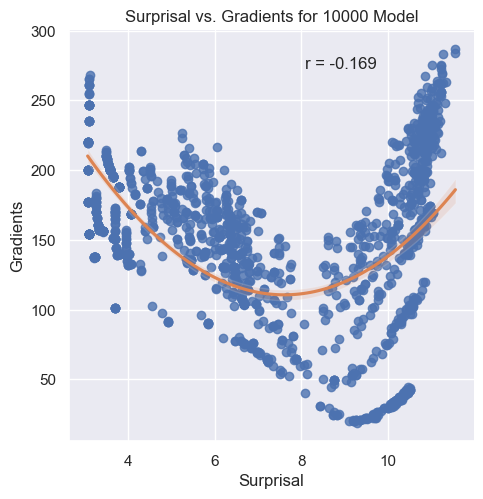
\includegraphics[width=\textwidth]{surprisal_vs_gradients/10000.png}
%     \end{subfigure}
%     \begin{subfigure}{0.4\textwidth}
%         \centering
%         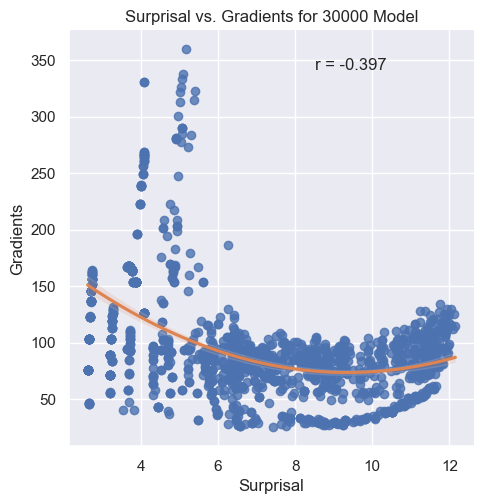
\includegraphics[width=\textwidth]{surprisal_vs_gradients/30000.png}
%     \end{subfigure}
% \end{figure*}
% \begin{figure*}[h]
% \centering
% \begin{subfigure}{0.4\textwidth}
%     \centering
%     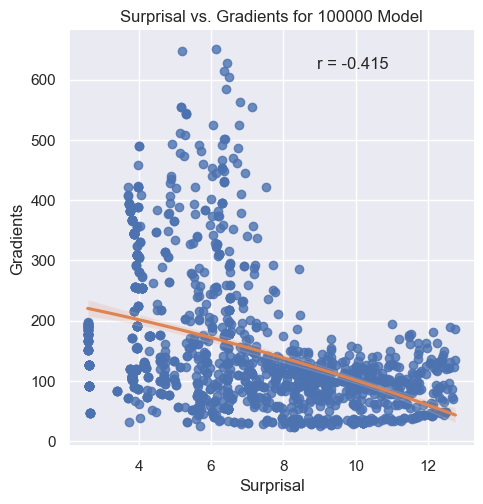
\includegraphics[width=\textwidth]{surprisal_vs_gradients/100000.png}
% \end{subfigure}
% \begin{subfigure}{0.4\textwidth}
%     \centering
%     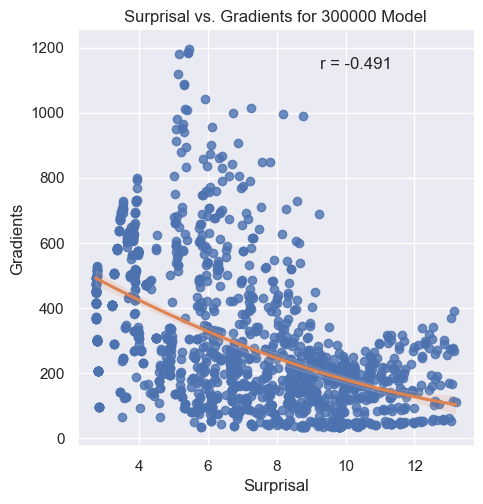
\includegraphics[width=\textwidth]{surprisal_vs_gradients/300000.png}
% \end{subfigure}
% \end{figure*}
% \begin{figure*}[h]
%     \centering
%     \begin{subfigure}{0.4\textwidth}
%         \centering
%         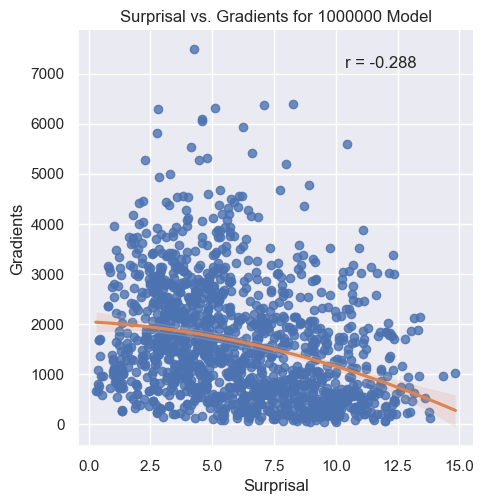
\includegraphics[width=\textwidth]{surprisal_vs_gradients/1000000.png}
%     \end{subfigure}
%     \begin{subfigure}{0.4\textwidth}
%         \centering
%         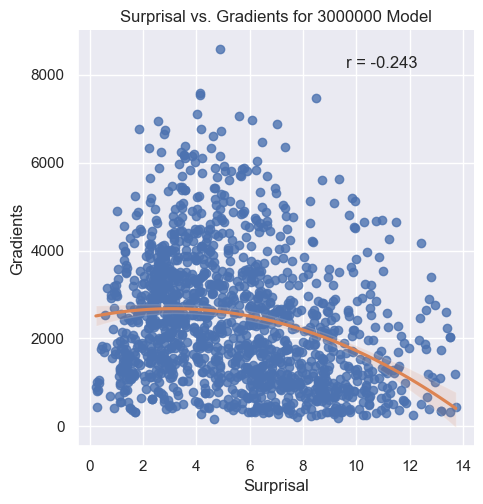
\includegraphics[width=\textwidth]{surprisal_vs_gradients/3000000.png}
%     \end{subfigure}
% \end{figure*}
% \begin{figure*}[h]
%     \centering
%     \begin{subfigure}{0.4\textwidth}
%         \centering
%         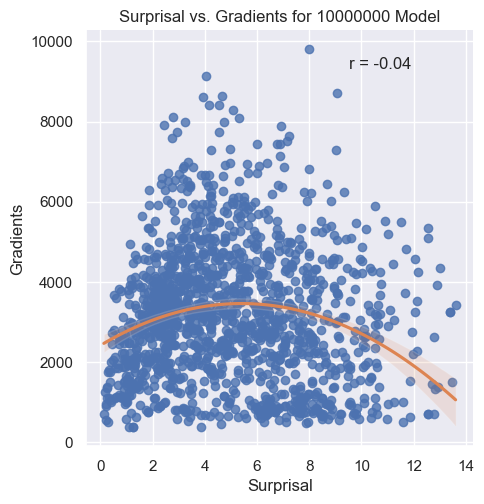
\includegraphics[width=\textwidth]{surprisal_vs_gradients/10000000.png}
%     \end{subfigure}
%     \begin{subfigure}{0.4\textwidth}
%         \centering
%         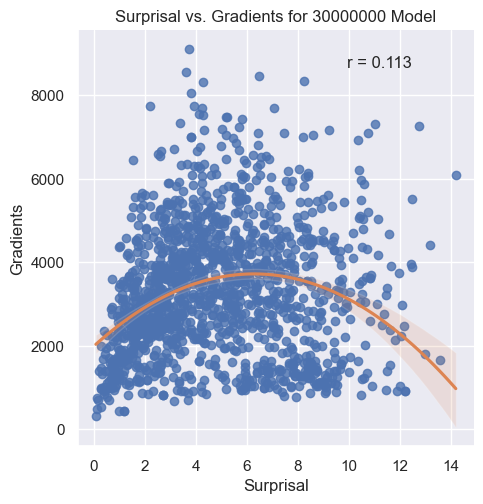
\includegraphics[width=\textwidth]{surprisal_vs_gradients/30000000.png}
%     \end{subfigure}
% \end{figure*}
% \begin{figure*}[h]
%     \centering
%     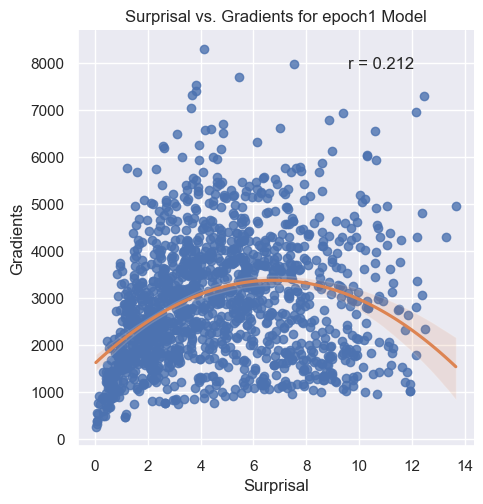
\includegraphics[width=0.4\textwidth]{surprisal_vs_gradients/epoch1.png}
% \end{figure*}

% \clearpage

% \section*{Appendix B: Plots of Model Gradients vs. Mean P600 Component}
% \begin{figure*}[h]
%     \centering
%     \begin{subfigure}{0.4\textwidth}
%         \centering
%         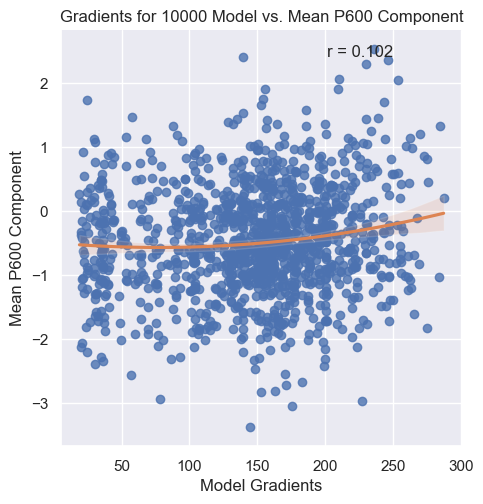
\includegraphics[width=\textwidth]{gradients_vs_p600/10000.png}
%     \end{subfigure}
%     \begin{subfigure}{0.4\textwidth}
%         \centering
%         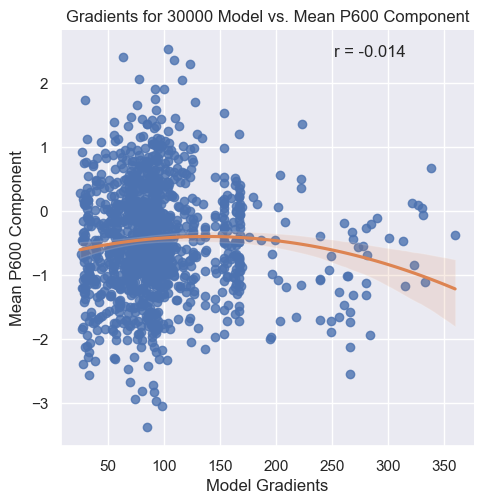
\includegraphics[width=\textwidth]{gradients_vs_p600/30000.png}
%     \end{subfigure}
% \end{figure*}
% \begin{figure*}[h]
% \centering
% \begin{subfigure}{0.4\textwidth}
%     \centering
%     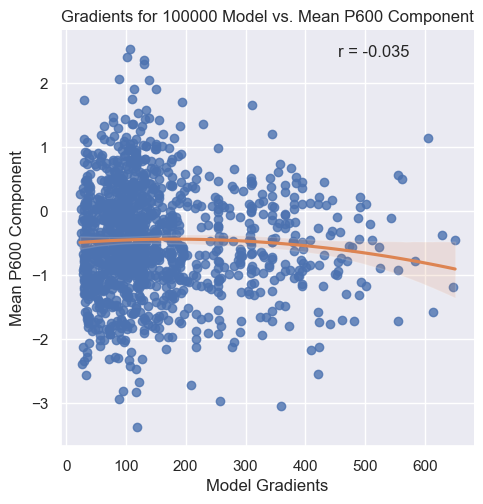
\includegraphics[width=\textwidth]{gradients_vs_p600/100000.png}
% \end{subfigure}
% \begin{subfigure}{0.4\textwidth}
%     \centering
%     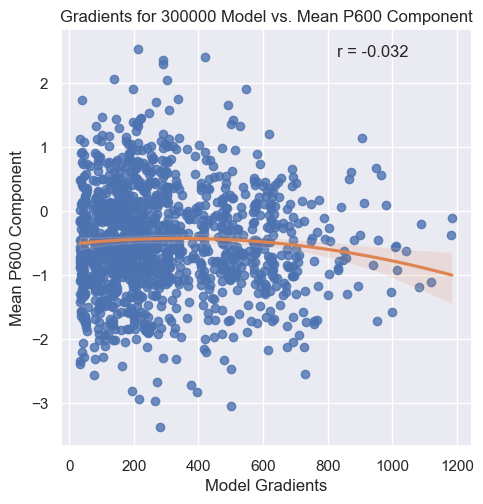
\includegraphics[width=\textwidth]{gradients_vs_p600/300000.png}
% \end{subfigure}
% \end{figure*}
% \begin{figure*}[h]
%     \centering
%     \begin{subfigure}{0.4\textwidth}
%         \centering
%         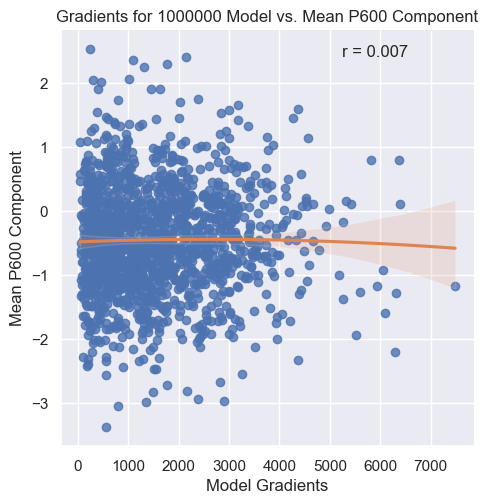
\includegraphics[width=\textwidth]{gradients_vs_p600/1000000.png}
%     \end{subfigure}
%     \begin{subfigure}{0.4\textwidth}
%         \centering
%         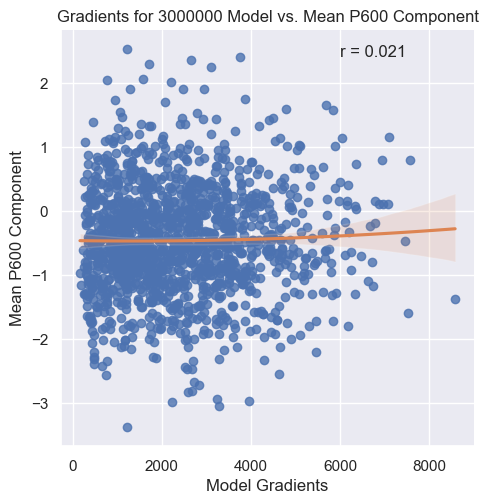
\includegraphics[width=\textwidth]{gradients_vs_p600/3000000.png}
%     \end{subfigure}
% \end{figure*}
% \begin{figure*}[h]
%     \centering
%     \begin{subfigure}{0.4\textwidth}
%         \centering
%         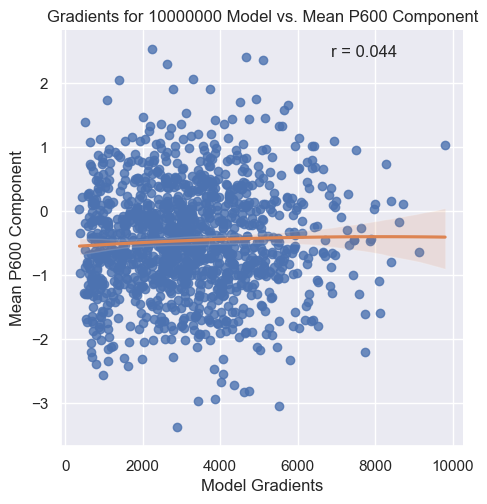
\includegraphics[width=\textwidth]{gradients_vs_p600/10000000.png}
%     \end{subfigure}
%     \begin{subfigure}{0.4\textwidth}
%         \centering
%         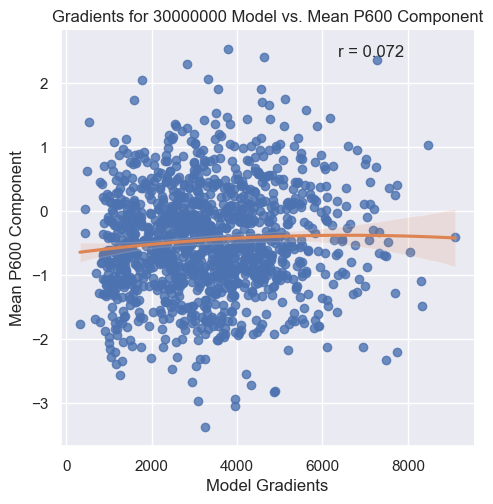
\includegraphics[width=\textwidth]{gradients_vs_p600/30000000.png}
%     \end{subfigure}
% \end{figure*}
% \begin{figure*}[h]
%     \centering
%     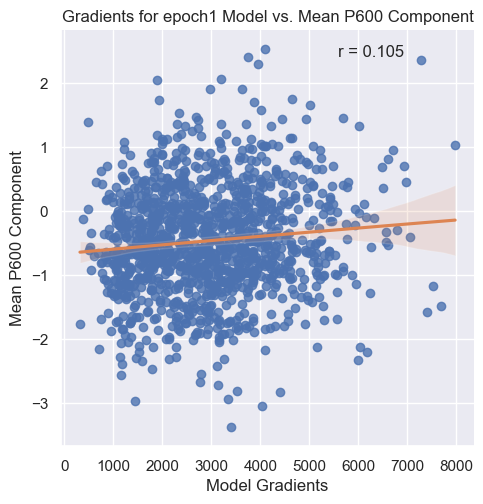
\includegraphics[width=0.4\textwidth]{gradients_vs_p600/epoch1.png}
% \end{figure*}

% \clearpage

% \section*{Appendix C: Plots of Model Surprisal vs. Mean P600 Component}
% \begin{figure*}[h]
%     \centering
%     \begin{subfigure}{0.4\textwidth}
%         \centering
%         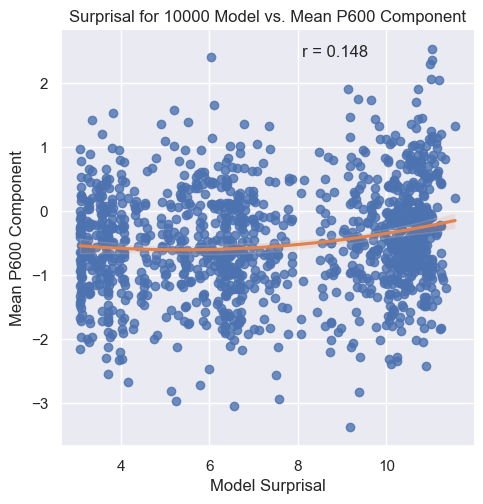
\includegraphics[width=\textwidth]{surprisal_vs_p600/10000.png}
%     \end{subfigure}
%     \begin{subfigure}{0.4\textwidth}
%         \centering
%         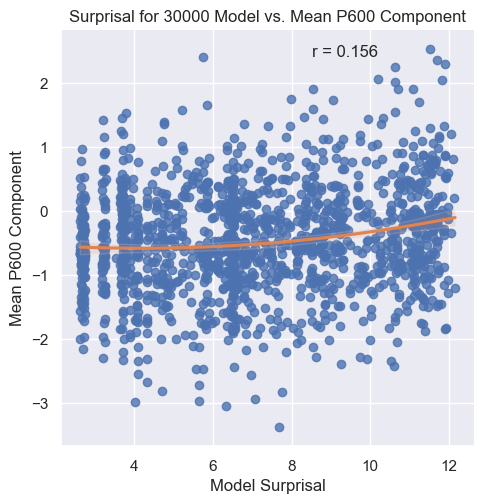
\includegraphics[width=\textwidth]{surprisal_vs_p600/30000.png}
%     \end{subfigure}
% \end{figure*}
% \begin{figure*}[h]
% \centering
% \begin{subfigure}{0.4\textwidth}
%     \centering
%     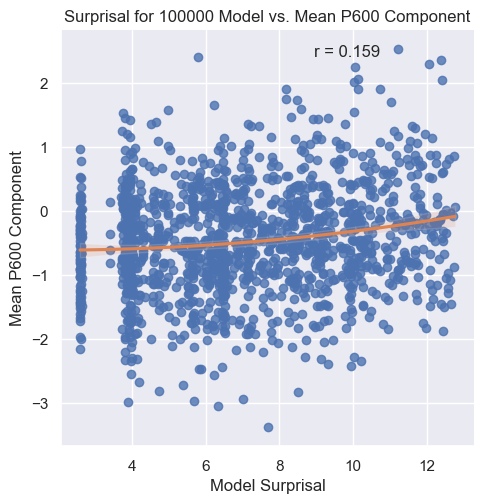
\includegraphics[width=\textwidth]{surprisal_vs_p600/100000.png}
% \end{subfigure}
% \begin{subfigure}{0.4\textwidth}
%     \centering
%     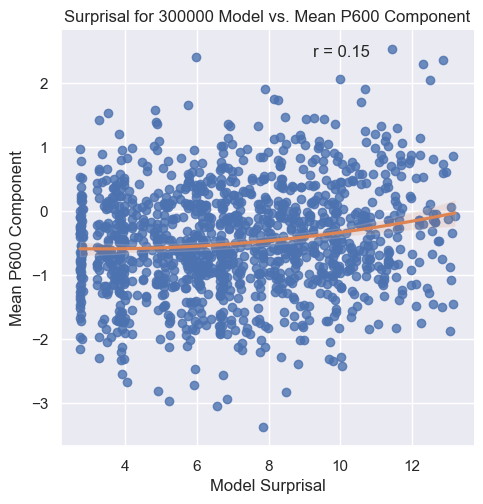
\includegraphics[width=\textwidth]{surprisal_vs_p600/300000.png}
% \end{subfigure}
% \end{figure*}
% \begin{figure*}[h]
%     \centering
%     \begin{subfigure}{0.4\textwidth}
%         \centering
%         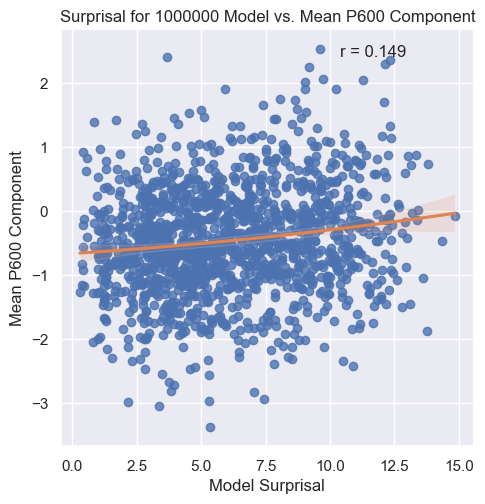
\includegraphics[width=\textwidth]{surprisal_vs_p600/1000000.png}
%     \end{subfigure}
%     \begin{subfigure}{0.4\textwidth}
%         \centering
%         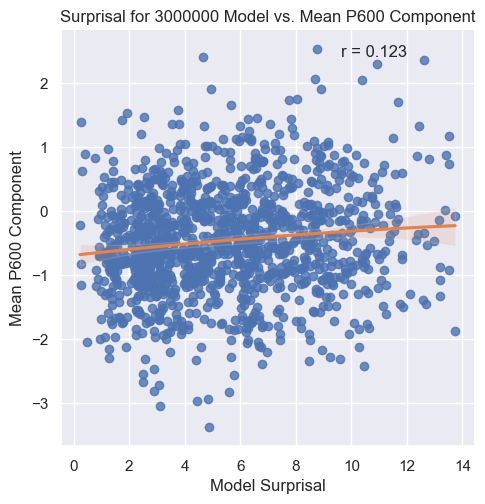
\includegraphics[width=\textwidth]{surprisal_vs_p600/3000000.png}
%     \end{subfigure}
% \end{figure*}
% \begin{figure*}[h]
%     \centering
%     \begin{subfigure}{0.4\textwidth}
%         \centering
%         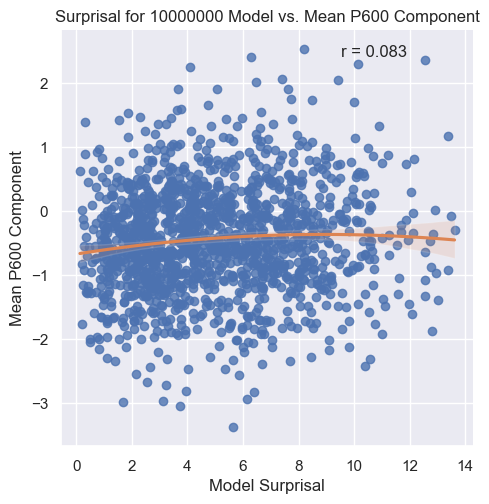
\includegraphics[width=\textwidth]{surprisal_vs_p600/10000000.png}
%     \end{subfigure}
%     \begin{subfigure}{0.4\textwidth}
%         \centering
%         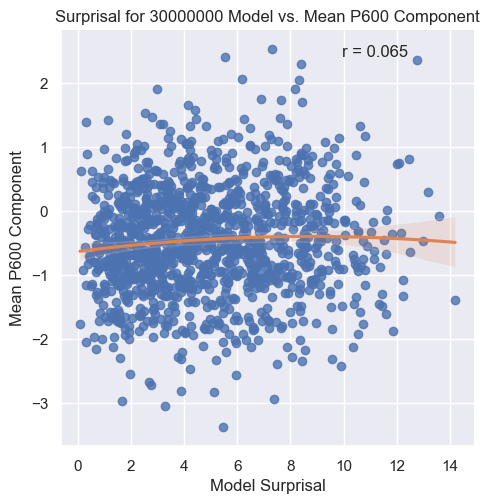
\includegraphics[width=\textwidth]{surprisal_vs_p600/30000000.png}
%     \end{subfigure}
% \end{figure*}
% \begin{figure*}[h]
%     \centering
%     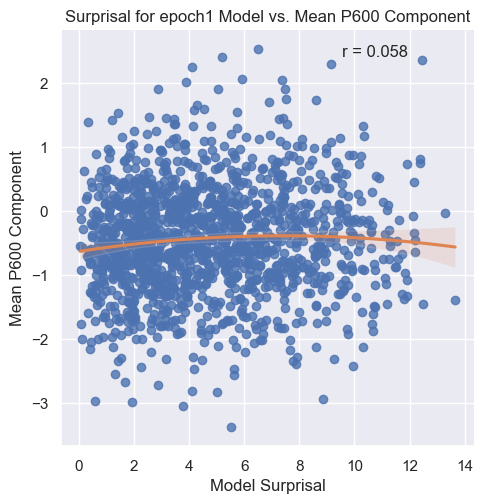
\includegraphics[width=0.4\textwidth]{surprisal_vs_p600/epoch1.png}
% \end{figure*}

\end{document}